\paragraph{Diagrammi UML}\mbox{}\\
Con l'obiettivo di rendere chiare le soluzioni progettuali utilizzate, è necessario l'utilizzo di {diagrammi UML}\ped{G}. Quest'ultimi devono essere realizzati utilizzando lo {standard}\ped{G} 2.0.

È richiesta la realizzazione di:
\begin{itemize}
	\item[•] \textbf{Diagrammi di attività}: descrivono un processo o un algoritmo;
	\item[•] \textbf{Diagrammi dei package}: per raggruppare elementi e fornire un {namespace}\ped{G} per gli elementi raggruppati;
	\item[•] \textbf{Diagrammi di sequenza}: rappresentano una sequenza di processi o funzioni;
	\item[•] \textbf{Diagrammi di classi}: rappresentano le classi utilizzate e le loro relazioni.
\end{itemize}
In caso vengano utilizzati dei {Design Pattern}\ped{G} sarà necessario accompagnarli con una descrizione ed un diagramma UML.

\subsubsection{Progettazione}\mbox{}
Dopo aver terminato il periodo di Analisi si passerà a quella di Progettazione che vede come 
protagonisti i \textit{Progettisti}, quest'ultimi hanno stabilito l'{architettura}\ped{G} logica 
da definire e i vari diagrammi che la rappresentano.
La Progettazione permette di: 
\begin{itemize}
\item[•] Ottimizzare l'uso delle risorse;
\item[•] Garantire la qualità del prodotto sviluppato;
\item[•] Suddividere il problema principale in tanti sotto problemi di complessità minore.
\end{itemize}

\paragraph{Architettura logica}\mbox{}\\
Bisogna definire un'architettura logica del prodotto che dovrà: 
\begin{itemize}
\item[•] Soddisfare i requisiti definiti nel documento di \AdR;
\item[•] Essere sicura in caso di malfunzionamenti o intrusioni;
\item[•] Essere {modulare}\ped{G} e formato da componenti riutilizzabili;
\item[•] Essere affidabile;
\item[•] Essere comprensibile per future manutenzioni.
\end{itemize}

\paragraph{Design Pattern}\mbox{}\\
I \textit{Progettisti} devono utilizzare il design pattern che ritengono più adatto al contesto per rendere l'applicazione più sicura ed efficiente possibile.
Ogni utilizzo di design pattern deve essere brevemente descritto ed accompagnato da un diagramma UML posto nella directory padre dei file sorgenti.

\subparagraph{Diagrammi di attività}\mbox{}\\
I diagrammi di attività sono rappresentati usando i formalismi definiti in UML 2. I principali sono riportati in seguito. Per indicare il consumo e la generazione di token, viene usata la seguente notazione: (T:token generati/token consumati).
\begin{itemize}
	\item \textbf{Nodo iniziale}: punto dal quale inizia l'esecuzione del processo. \`E rappresentato da un pallino nero (T:1/0);
	\item \textbf{Activity}: azione elementare svolta dal programma. Si rappresenta con un rettangolo che ne contiene una descrizione il più sintetica possibile (T:1/1);
	\item \textbf{Branch}: punto di decisione. Il flusso può intraprendere solo uno di n rami. Si rappresenta mediante un rombo con una freccia entrante e n uscenti. Ogni ramo è accompagnato da una \textit{guardia}, un'etichetta fra parentesi quadre che ne descrive la condizione;
	\begin{figure}[H]
		\centering
		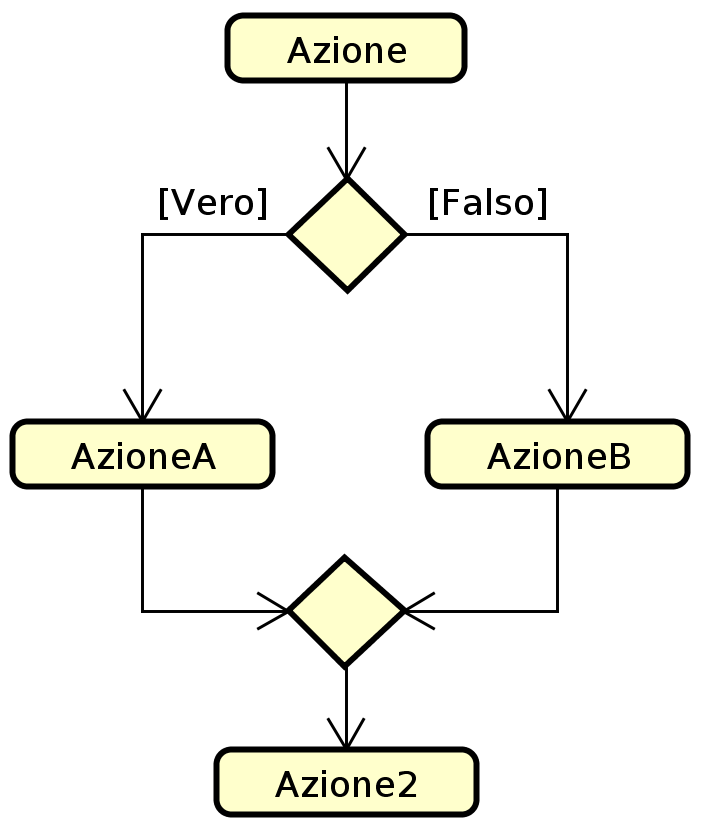
\includegraphics[width=6cm,keepaspectratio]{img/mergeBranch.png}
		\caption{Merge e branch}
	\end{figure}
	\item \textbf{Merge}: punto in cui rami derivanti da un branch si uniscono. Si rappresenta come un rombo (T:1/1);
	\item \textbf{Fork}: punto da cui partono 2 o più processi paralleli. Si rappresenta come una spessa linea orizzontale o verticale, con una freccia entrante e n uscenti (T:1/N);
	\item \textbf{Join}: punto in sincronizzazione di processi paralleli. Si rappresenta come un Fork, ma con n frecce entranti e una uscente. Può essere accompagnato da un'espressione booleana che ne specifica il funzionamento (T:N/1);
	\item \textbf{Pin}: passaggio di parametri fra activity. Si rappresenta tramite un quadratino dal quale escono o entrano delle frecce. \'E accompagnato dal tipo del parametro trasferito, posto a fianco;
	\item \textbf{Subactivity}: indica che l'azione che l'activity svolge è descritta più in dettaglio in un diagramma separato. Una sotto-attività ha sempre un input e un output. Si indica con box simile a quello dell'activity che presenta un piccolo tridente in basso a sinistra (T:1/1);
	\item \textbf{Partizioni}: forniscono una responsabilità all'esecuzione delle azioni. Si indicano tramite delle linee verticali che dividono il diagramma in più partizioni;
	\item \textbf{Segnali}: rappresentano l'invio/ricezione di eventi a/da processi esterni. Si rappresentano attraverso un rettangolo con una concavità triangolare per la ricezione, e tramite un rettangolo con una convessità triangolare per l'invio. Entrambi contengono una breve descrizione del segnale;
	\item \textbf{Timeout}: modellano dei timeout. Si presentano come una clessidra, possono avere frecce entranti e uscenti, e sono accompagnati dalla descrizione in linguaggio naturale dell'intervallo di tempo che deve trascorrere;
	\item \textbf{Eventi Ripetuti}: modellano degli eventi che si ripetono nel tempo, generando un token ad ogni ripetizione. Possono avere solo frecce uscenti, e si rappresentano con una descrizione dell'intervallo della ripetizione;
	\item \textbf{Nodi di fine flusso}: rappresenta la morte di un ramo di esecuzione. Si rappresenta tramite un cerchio con una X (T:1/0);
	\item \textbf{Nodo finale} : rappresenta la fine dell'esecuzione di un processo. Si rappresenta tramite un cerchio pieno racchiuso in una circonferenza di raggio maggiore (T:0/1).
	\begin{figure}[H]
		\centering
		
\includegraphics[width=6cm,keepaspectratio]{img/nodi.png}
		\caption{Nodi, da sinistra a destra: iniziale, finale, di di fine flusso.}
	\end{figure}
\end{itemize}

\subparagraph{Diagrammi di sequenza}\mbox{}\\
Ogni diagramma di sequenza avrà un senso di lettura verticale dall’alto al basso, il verso indica lo scorrere del tempo.  Gli oggetti coinvolti verranno rappresentati tramite un rettangolo, al cui interno si troverà un nome per identificarli nel formato di istanza: \textbf{NomeClasse}.\\ Sotto ad ogni istanza si troverà una linea della vita tratteggiata, che sarà sormontata in alcuni tratti da una barra di attivazione che indica i momenti in cui l’oggetto è attivo.  Da una barra di attivazione partiranno delle frecce, che rappresentano un messaggio o segnale, verso la linea della vita di oggetti già instanziati, in alternativa, verso una nuova istanza di classe per crearla.  In particolare, verranno utilizzati i seguenti tipi di frecce:
\begin{itemize}
\item Freccia piena, per indicare un messaggio sincrono: corrisponde alla chiamata di un metodo. Sopra tale freccia si dovrà specificare il metodo invocato secondo il formato:
\begin{center}
\texttt{nomeMetodo(lista parametri formali)}
\end{center} 

\item Freccia, per indicare un messaggio asincrono, chi invoca il metodo non attendendo il return; 

\item Freccia tratteggiata, per indicare il ritorno di un metodo chiamato. Sopra tale freccia si dovrà indicare il tipo di ritorno secondo il formato: \texttt{TipoRitorno};

\item Freccia trattegiata sormontata da \texttt{<<create>>}, indica la creazione di un nuovo oggetto e termina sempre in un rettangolo che ne contiene il nome nel formato \texttt{istanza: NomeClasse};

\item Freccia piena sormontata da \texttt{<<destroy>>}, indica la distruzione di un oggetto e
termina sempre in una X, nella quale muore anche la linea della vita dell’oggetto.
\end{itemize}
Sarà inoltre possibile determinare sui diagrammi di sequenza dei frame di interazione
associati ad una guardia o condizione:
\begin{itemize}
\item \textbf{alt}: indica dei frammenti in alternativa fra loro, verrà eseguito quello per cui la
guardia è verificata;
\item \textbf{opt}: indica un frammento che viene eseguito solo se la guardia è specificata;
\item \textbf{par}: indica frammenti eseguiti in parallelo;
\item \textbf{loop}: indica un frammento che viene eseguito più volte, la condizione di arresto del
ciclo è la guardia;
\item \textbf{region}: indica un frammento critico che deve essere eseguito in mutua esclusione.
\end{itemize}

	\begin{figure}[H]
		\centering
		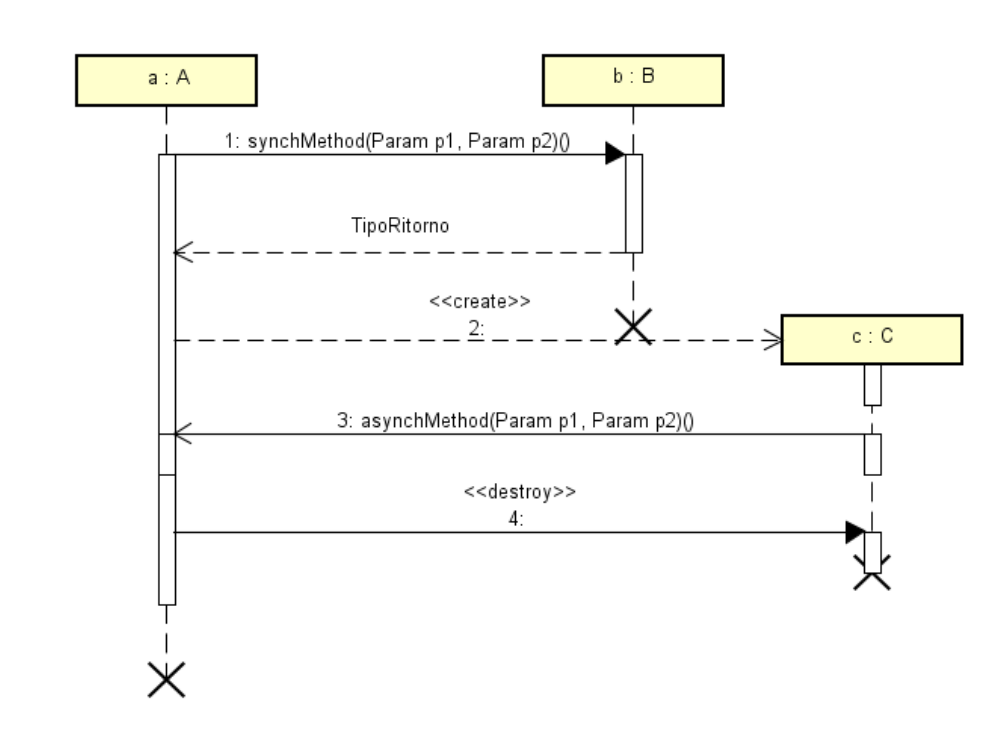
\includegraphics[width=13cm,keepaspectratio]{img/DiagrammaDiSequenza.png}
		\caption{Diagramma di sequenza con tutti i tipi di segnale}
	\end{figure}





\subparagraph{Diagrammi dei package}\mbox{}\\
Ogni package verrà rappresentato tramite un rettangolo con un’etichetta per il nome, che dovrà contenere i diagrammi delle classi appartenenti al package ed eventuali sotto-package. Le dipendenze fra i vari package dovranno
essere segnalate con una freccia tratteggiata. Tale freccia, disegnata dal package A al package B, indica una dipendenza di A ne confronti di B. Si devono evitare dipendenze cicliche.
\begin{figure}[H]
		\centering
		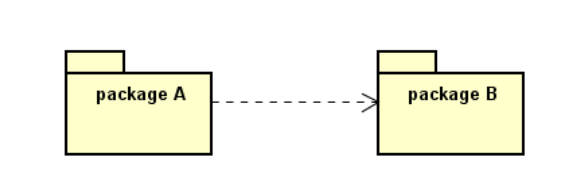
\includegraphics[width=8cm,keepaspectratio]{img/DiagrammaFraPackages.png}
		\caption{Esempio di diagramma dei package}
	\end{figure}


\subparagraph{Diagrammi delle classi}\mbox{}\\
Tutte le classi devono seguire l'ultima specifica UML 2.X. Allo stesso modo ogni relazione o dipendenza fra classi deve essere indicata con l'opportuna notazione.
Le classi rappresentate nei diagrammi devono avere lo stesso nome di quelle nel codice vero e proprio, così come attributi e nomi dei metodi. È possibile, a seconda del livello di dettaglio del diagramma, omettere metodi o attributi che non risultino fondamentali per la comprensione del diagramma stesso (come, ad esempio, \texttt{getters} e \texttt{setters}).
\begin{figure}[H]
		\centering
		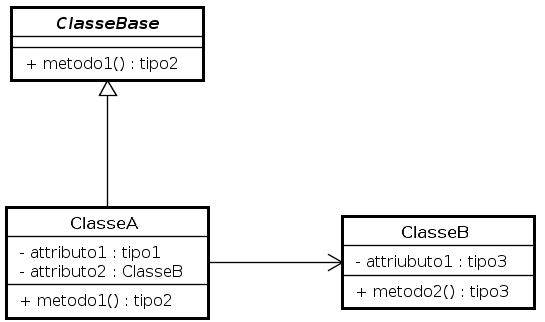
\includegraphics[width=8cm,keepaspectratio]{img/DiagrammaClassi.png}
		\caption{Esempio di diagramma delle classi}
	\end{figure}




\subsubsection{Qualità}

\paragraph{Classificazione dei test}\mbox{}\\

Ogni Test è strutturato come segue:
\begin{itemize}
\item Codice identificativo; 
\item Descrizione;
\item Stato. 
\end{itemize}
Per ciascun test è assegnato un codice identificativo la cui sintassi segue il seguente
formalismo:
\begin{center}
\textbf{T\{tipo\}\{codiceIdentificativo\}}
\end{center}
Dove: 
\begin{itemize}
\item \textbf{lettera}: identifica uno dei seguenti tipi di test:
	\begin{itemize}
		\item \textbf{U}: test di unità; 
		\item \textbf{I}: test di integrazione; 
		\item \textbf{S}: test di sistema.
	\end{itemize}
\item \textbf{codiceIdentificativo}: assume i seguenti valori in base al tipo di test:
	\begin{itemize}
	\item \textbf{codiceNumerico}: associato ai test di unità e di integrazione, è un codice
progressivo di tre cifre che parte da 001;
	\item \textbf{codiceRequisito}: associato ai test di sistema. Identifica il codice univo-
co associato ad ogni requisito descritto nel documento Analisi dei Requisiti
v3.0.0.
	\end{itemize}
\end{itemize}	
Inoltre lo Stato del test può assumere i seguenti valori:
\begin{itemize}
\item Non implementato;  
\item Superato; 
\item Non superato. 
\end{itemize}

\paragraph{Test di unità}\mbox{}\\
Devono essere definiti dei testi di unità necessari a garantire che tutte le componenti del sistema funzionino correttamente.

\paragraph{Test di integrazione}\mbox{}\\
Devono essere definite le classi di verifica necessarie a garantire che tutte le componenti del sistema funzionino correttamente.

\paragraph{Test di sistema}\mbox{}\\
Richiede che i vari componenti del sistema vengano integrati al fine di garantire che tutte le componenti del sistema funzionino correttamente.

\subsubsection{Codifica}
In questa sezione vengono descritte le norme che i \textit{Programmatori} devono seguire con l'obiettivo di scrivere codice leggibile, affidabile e manutenibile.

\paragraph{Linguaggi e Framework}\mbox{}\\
Lo sviluppo del progetto didattico richiede l'uso di diversi framework e linguaggi di programmazione, ognuno mirato ad uno scopo preciso:
\begin{itemize}
	\item \textbf{JavaScript:} viene adottato Javascript alla specifica ES6 per lo sviluppo di gran parte della backend e della frontend;
	\item \textbf{React:} viene adottato il framework React 16.8 per lo sviluppo della parte di frontend;
	\item \textbf{Java:} viene adottato Java con le specifiche del JDK 11 per lo sviluppo del modulo Server;
	\item \textbf{Spring:} viene adottato il framework Spring 2.0.5 per facilitare lo sviluppo del modulo sopracitato, avvalendosi solo del modulo RESTful. Vedi paragrafo \hyperref[sec:Spring]{§3.2.5.12}.
	\item \textbf{Spring Data MongoDB}: viene adottato il framework Spring Data MongoDB per interrogare e aggiornare le informazioni presenti nel database, vedi paragrafo \hyperref[sec:DataMongoDB]{§3.2.5.13}.
\end{itemize}


\paragraph{Stile di codifica}\mbox{}\\
Al fine di produrre codice uniforme, leggibile e manutenibile è richiesto che vengano rispettate
le seguenti convenzioni:
\begin{itemize}
\item[•] I nomi utilizzati devono essere chiari, descrittivi rispetto alla loro funzione e in inglese;
\item[•] Evitare nomi troppo simili tra loro che possano creare difficoltà nella comprensione del codice;
\item[•] Deve essere presente almeno un breve commento descrittivo per ogni classe e metodo;
\item[•] I commenti devono essere scritti in lingua inglese senza utilizzare abbreviazioni o altre ambiguità;
\item[•] Le modifiche al codice devono sempre riflettersi sui relativi commenti;
\item[•] Evitare commenti superflui o  inappropriati;
\item[•] Codifica dei file UTF-8.
\end{itemize}

 \paragraph{Intestazione}\mbox{}\\
Ogni file deve presentare un'intestazione con le seguenti informazioni:
\begin{itemize}
\item @path: percorso e nome del file;
\item @author: nome e cognome dell'autore o autori separati da una virgola;
\item @date: data ultima modifica;
\item @description: breve descrizione del contenuto del file.
\end{itemize}

\paragraph{Java Style Code}\mbox{}\\
Lo stile di codifica fa riferimento al Gooogle style code reperibile:
\begin{center}
\url{https://google.github.io/styleguide/javaguide.html}
\end{center}
Sono di particolare rilevanza §4 e §5, ovvero:
\begin{itemize}
\item \href{https://google.github.io/styleguide/javaguide.html#s4.1.3-braces-empty-blocks}{Empty blocks: may be concise}\\
\begin{lstlisting}[frame=single, language=java]
  // This is acceptable
  void doNothing() {}

  // This is equally acceptable
  void doNothingElse() {
  }
 \end{lstlisting}
\item \href{https://google.github.io/styleguide/javaguide.html#s4.5.1-line-wrapping-where-to-break}{Where to break}

\item \href{https://google.github.io/styleguide/javaguide.html#s4.8.2-variable-declarations}{Variable declarations}
\item \href{https://google.github.io/styleguide/javaguide.html#s4.8.5-annotations}{Annotations}
\item \href{https://google.github.io/styleguide/javaguide.html#s4.8.6-comments}{Comments}\\
\begin{lstlisting}[frame=single, language=java]
/*
 * This is          // And so           /* Or you can
 * okay.            // is this.          * even do this. */
 */
 \end{lstlisting}
\end{itemize}
Per quanto riguarda il paragrafo §5 è necessaria la lettura completa.
Al fine di garantire l'adozione del stylecode di Google è possibile impostare Eclipse IDE con lo style appropriato.
Lo style in formato {XML}\ped{G} per gli IDE è disponibile al seguente link:
\begin{center}
\href{https://github.com/google/styleguide}{Styleguide by Google}
\end{center}
Per vedere come importare gli stili di codifica fare riferimento a §3.2.6.4.

\paragraph{JavaScript Style Code}\mbox{}\\
Lo stile di codifica utilizzato per JSX di React è quello fornito da Airbnb e reperibile al link:
\begin{center}
\href{https://github.com/airbnb/javascript/tree/master/react}{Styleguide for React by Airbnb}
\end{center}
Seguono alcune convenzioni per una più facile fruibilità: 
\begin{itemize}
	\item Vanno utilizzati 2 spazi per ogni livello di indentazione, inoltre dopo la chiusura delle parentesi tonde dell'if è necessario uno spazio:\\
	\begin{lstlisting}[frame=single, language=JavaScript]
function() {
  let name;
}
	\end{lstlisting}
	\item \uppercase{è} necessario uno spazio prima della parentesi apertura del blocco per le seguenti istruzioni: \texttt{if}, \texttt{while}, \texttt{switch} e \texttt{do}.
	\item Il nome delle classi deve utilizzare la PascalCase notation:
		\begin{lstlisting}[frame=single, language=JavaScript]
//YES
class Animal {
}

//NO
class animal {
}
	\end{lstlisting}
	\item Utilizzare PascalCase per i componenti React e la notazione camelCase le loro istanze:
		\begin{lstlisting}[frame=single, language=JavaScript]
// bad
import reservationCard from './ReservationCard';

// good
import ReservationCard from './ReservationCard';

// bad
const ReservationItem = <ReservationCard />;

// good
const reservationItem = <ReservationCard />;
	\end{lstlisting}
	\item Utilizzare i doppi apici (") per gli attributi JSX, un apice singolo (') per tutti gli altri file JS:
		\begin{lstlisting}[frame=single, language=JavaScript]
// bad
<Foo bar='bar' />

// good
<Foo bar="bar" />

// bad
<Foo style={{ left: "20px" }} />

// good
<Foo style={{ left: '20px' }} />
	\end{lstlisting}
	\item Racchiudere i tag JSX all'interno di parentesi quando questi occupano più di una linea:
			\begin{lstlisting}[frame=single, language=JavaScript]
// bad
render() {
  return <MyComponent variant="long body" foo="bar">
           <MyChild />
         </MyComponent>;
}

// good
render() {
  return (
    <MyComponent variant="long body" foo="bar">
      <MyChild />
    </MyComponent>
  );
}

	\end{lstlisting}
	\item Utilizzare le arrow-function per gestire le variabili locali:
		\begin{lstlisting}[frame=single, language=JavaScript]
function ItemList(props) {
  return (
    <ul>
      {props.items.map((item, index) => (
        <Item
          key={item.key}
          onClick={(event) => doSomethingWith(event, item.name, index)}
        />
      ))}
    </ul>
  );
}
		\end{lstlisting}
		\item Sinstassi per creare componenti correttamente:
		\begin{lstlisting}[frame=single, language=JavaScript]
// bad
React.createClass({
  _onClickSubmit() {
    // do stuff
  },

  // other stuff
});

// good
class extends React.Component {
  onClickSubmit() {
    // do stuff
  }

  // other stuff
}
	\end{lstlisting}
\end{itemize}


\subsubsection{Regole comuni}
\paragraph{Ricorsione}\mbox{}\\
La ricorsione va sempre evitata se possibile. Per ogni funzione ricorsiva è necessario fornire
una prova di terminazione nei commenti.

\paragraph{Variabili globali}\mbox{}\\
L'uso di variabili globali va sempre evitato se possibile.

\paragraph{Funzioni anonime}\mbox{}\\
Per definire funzioni anonime bisogna usare la notazione a freccia, sono più concise e
mantengono il contesto del {this}\ped{G}.

\paragraph{Lunghezza massima righe}\mbox{}\\
La lunghezza massima per ciascuna riga di codice è di 100 caratteri, si suggerisce comunque
ove possibile di rimanere entro gli 80 caratteri per favorire la leggibilità.

\paragraph{Regole di denominazione}\mbox{}\\
\begin{itemize}
\item Utilizzare nomi descrittivi;
\item Utilizzare la camelCase\ped{G} per nominare oggetti, funzioni e istanze;
\item Utilizzare la PascalCase\ped{G} solamente per le classi e i costruttori;
\item Non utilizzare trattini bassi prefissi o postfissi.
\end{itemize}

\paragraph{Codetags}\mbox{}\\
I codetags sono delle parole chiavi informali all'interno dei commenti per segnalare
dei problemi, note o delle parti di codice ancora da fare. La struttura `e la seguente: \\
<tag>: <descrizione in una singola linea>\\
I tag che verranno utilizzati sono:
\begin{itemize}
\item \textbf{TODO}: qualcosa che va completato;
\item \textbf{NOTE}: annotazioni particolari;
\item \textbf{FIXME}: qualcosa che va risolto perchè non funzionante;
\item \textbf{HACK}: qualcosa che funziona ma andrebbe migliorato.
\end{itemize}
Potranno essere usati all’interno di commenti blocco o inline. Sono supportati da
molti IDE ed editor moderni.

\subsubsection{Feature branch}
Per l'attività di codifica si utilizza il modello feature branch, ovvero ogni funzionalità viene creata e testata in un branch a parte prima di essere mergiata, ovvero integrata, all'interno dell'applicativo.
I punti forti di questo modello sono:\\
\begin{itemize}
\item Usare un branch per feature/caratteristica;
\item L'incapsulamento consente di lavorare senza disturbare la base di codice principale;
\item Consente una collaborazione più semplice;
\item Unisce e mappa i conflitti concettuali: più facile da tracciare.
\end{itemize}
\begin{figure}[H]
\centering
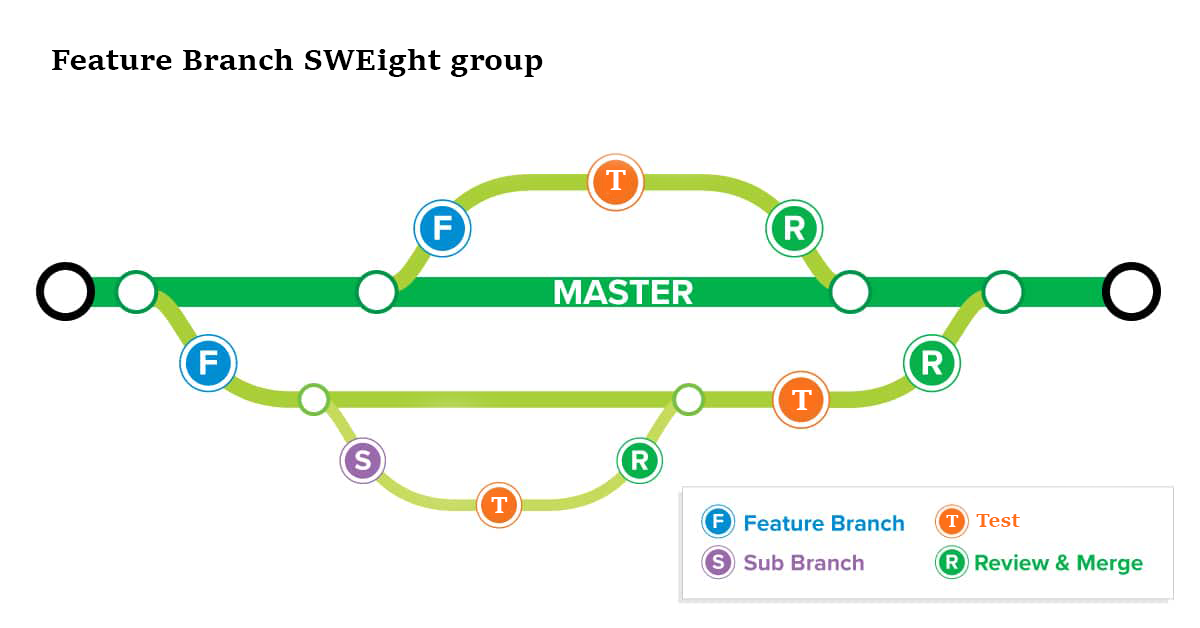
\includegraphics[width=14cm,keepaspectratio]{img/pan-featurebranch.png}
\caption{Panoramica feature branch}
Immagine tratta da www.revelry.co
\end{figure}
\begin{figure}[H]
\centering
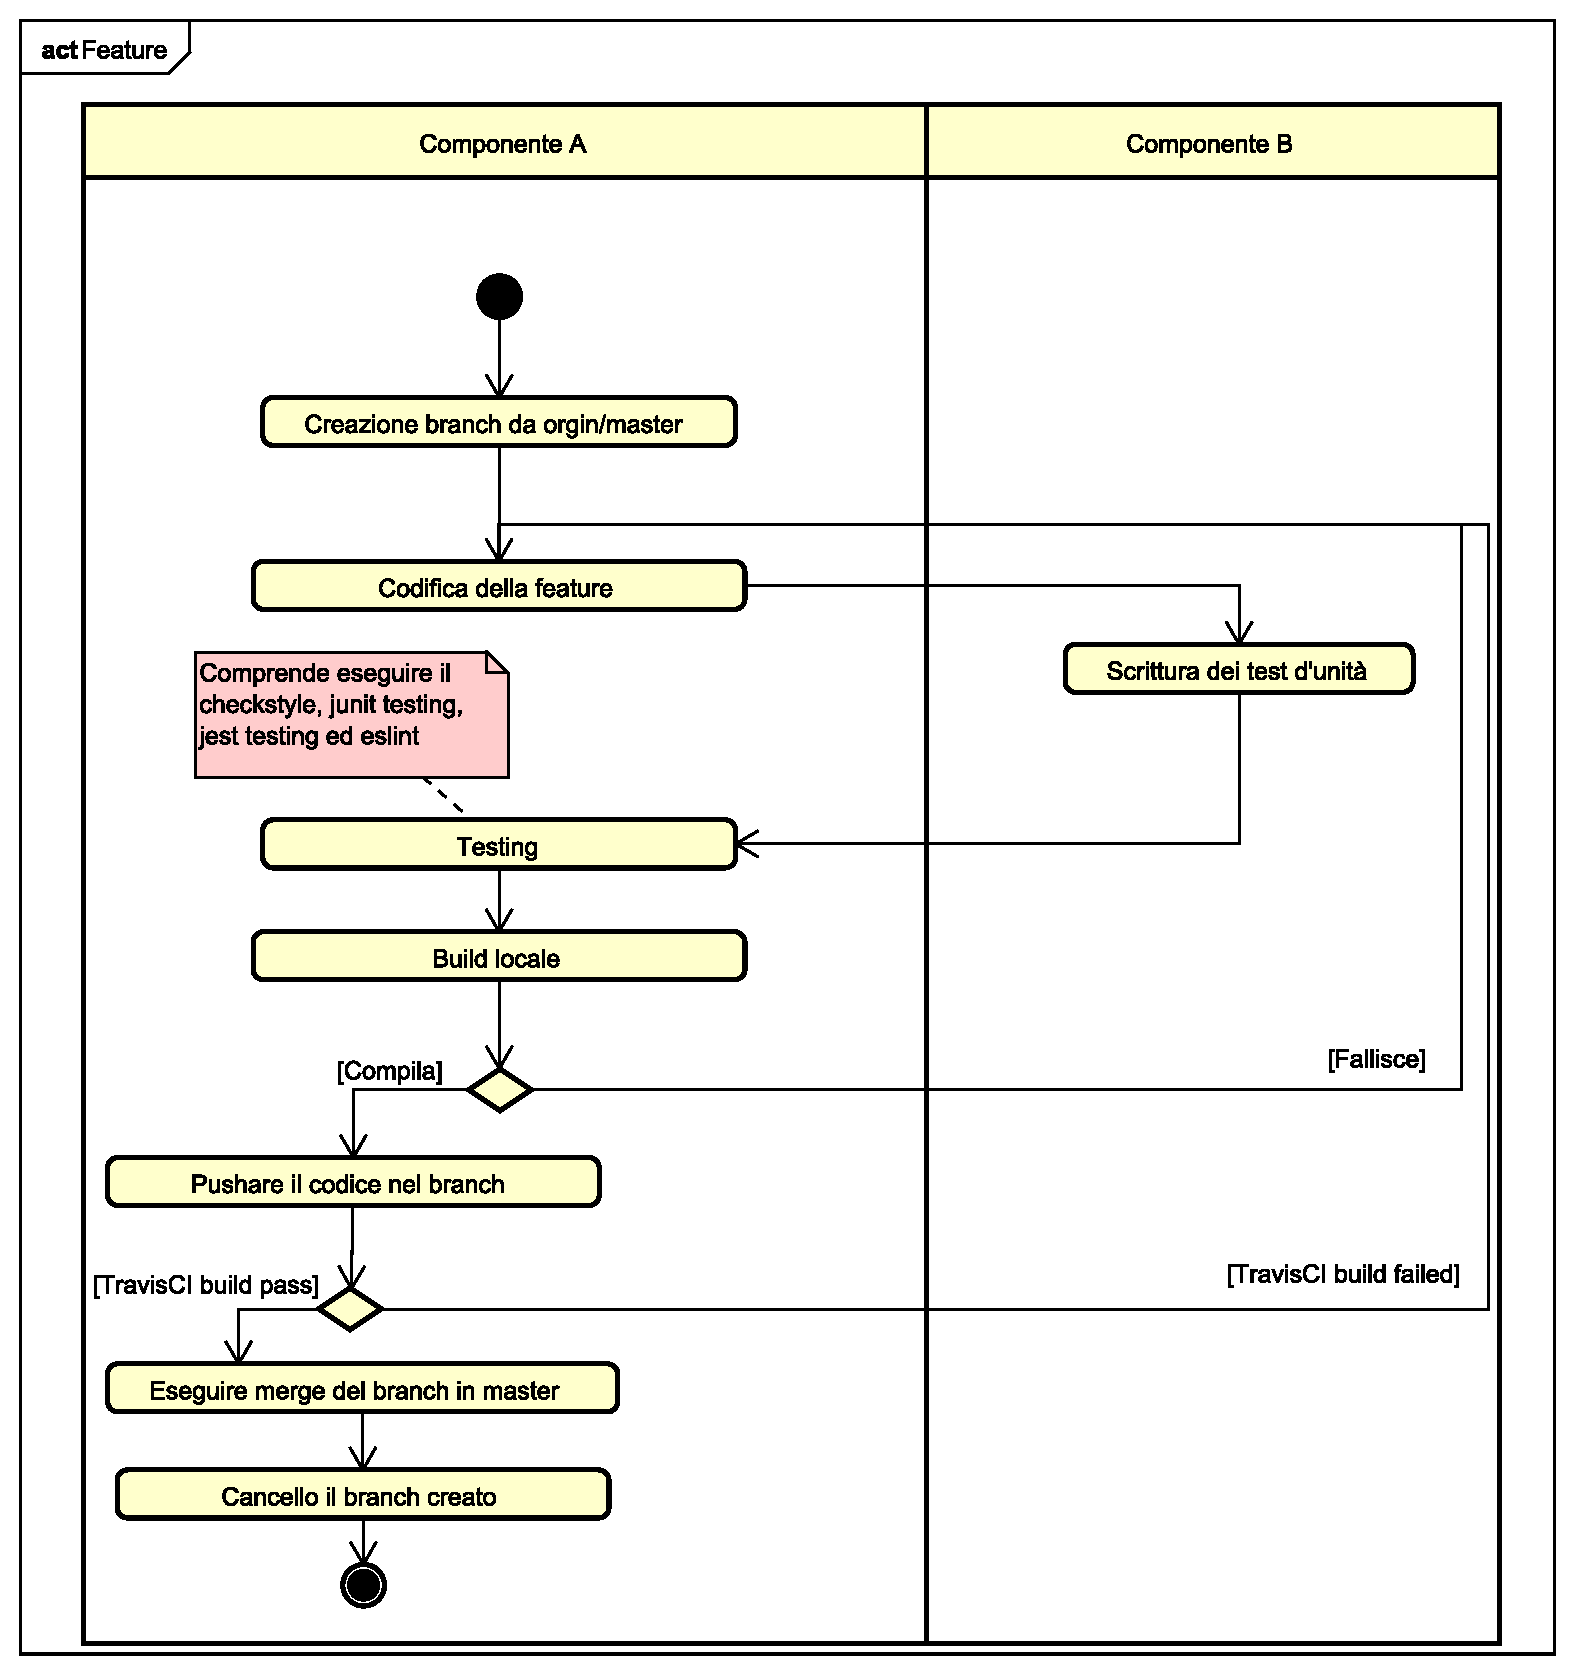
\includegraphics[width=17cm,keepaspectratio]{img/Feature.pdf}
\caption{Diagramma di sequenza feature branch, con il termine componente si fa riferimento a due elementi del gruppo}
\end{figure}
\subsubsection{Strumenti di supporto}
\paragraph{RQConnect}\mbox{}\\ \label{sec:Trac}
Il tracciamento dei requisiti e dei casi d’uso avviene attraverso la piattaforma 
\textit{RQConnect}, installata su un server {Firebase}\ped{G} ad hoc per il gruppo \gruppo.
 È  un tool sviluppato da un componente del gruppo in occasione di questo progetto e 
 liberamente disponibile su GitHub.\\ È possibile aggiungere requisiti e casi d’uso 
 alla piattaforma e successivamente collegarli tra di loro, la schermata principale è 
 divisa in due colonne, in quella a sinistra c’è l’elenco dei requisiti e in quella a 
 destra i casi d’uso, cliccando su un elemento si apre una vista dettagliata nella quale 
 è possibile leggere i dettagli e collegare l’elemento, cliccando sul pulsante \textit{risolvi} si 
 apre una finestra dalla quale è possibile selezionare gli elementi da collegare con l’aiuto 
 di un menu a tendina.\\Una volta completato l’inserimento ed il collegamento è possibile scaricare 
 l’intera lista in tabella \LaTeX.

\paragraph{Visual studio code}\mbox{}\\
L'{IDE}\ped{G} scelto per lo sviluppo è {Visual studio code}\ped{G}, versione: 1.31 disponibile al seguente link:
\begin{center}
	\url{https://code.visualstudio.com/Download};
\end{center}
Esso è stato scelto principalmente perché gratuito, include supporto per il debugging e un controllo Git integrato oltre al {Syntax highlighting}\ped{G}, {IntelliSense}\ped{G}, {Snippet}\ped{G} e {code refactoring}\ped{G}.\\
Si farà riferimento ai seguenti linguaggi, piattaforme, librerie e framework:
\begin{itemize}
	\item[•]{JavaScript}\ped{G} 1.8.5;
	\item[•]{HTML5}\ped{G};
	\item[•]{Node.js}\ped{G} 10.15.1;
	\item[•]{React}\ped{G} 16.8.1;
	\item[•]{Bootstrap}\ped{G} 4.3.0.
\end{itemize}

I plugin utilizzati sono:
\begin{itemize}
	\item \textbf{Prettier - Code formatter}: per la formattazione automatica del codice.
	Per settare la formattazione automatica al salvataggio del file si deve:
	\begin{itemize}
		\item Premere CMD + Shift + P;
		\item Andare su Open User Settings;
		\item Andare in Text Editor > Formatting;
		\item Spuntare la casella Format on save.
	\end{itemize}
	\item \textbf{Simple React Snippet}: per facilitare la scrittura del codice con semplici comandi come:
	\begin{itemize}
		\item \textbf{Imrc}: Per l'import;
		\item \textbf{Cc}: Per creare le classi;
		
	\end{itemize}
\end{itemize}

\paragraph{Docker}\mbox{}\\
Lo strumento scelto per contenere la libreria di pos-tagging con il relativo server {TCP/IP}\ped{G} è Docker. Esso permette di inserire l'applicativo scritto in {C++}\ped{G} all'interno di contenitori software, fornendo un'astrazione aggiuntiva grazie alla virtualizzazione a livello di sistema operativo di Linux.
Per installare Docker nella versione 18.09, è necessario installare Docker Desktop in Windows 10 Pro o Enterprise e in MacOS:
\begin{center}
\url{https://www.docker.com/products/docker-desktop}
\end{center}
Mentre in Ubuntu Linux è consigliato seguire la seguente guida: \href{https://www.digitalocean.com/community/tutorials/how-to-install-and-use-docker-on-ubuntu-18-04}{"How To Install and Use Docker on Ubuntu 18.04"}.
Il Dockerfile contiene la configurazione per la compilazione e l'installazione dell'applicativo.\\
Per generare l'immagine è necessario eseguire il seguente comando:
\begin{center}
	\texttt{\# docker build --tag=freeling:alpha .}
\end{center}
Successivamente quest'ultima potrà essere eseguita con il comando:	
\begin{center}
	\texttt{\# docker run -it --rm -p 50005:50005 freelingserver:alpha analyze -f es.cfg --server -p 50005}
\end{center}
L'istruzione crea un'istanza dell'immagine che è in attesa di richieste sulla porta 50005 che analizza frasi scritte in lingua spagnola.
Per permettere di analizzare frasi in più lingue creare istanze diverse con il comando precedente (\texttt{docker run}) sostituendo \texttt{es.cfg} con la lingua d'interesse, ad esempio: \texttt{it.cfg}.\\
Alcune delle lingue disponibili sono: 
\begin{itemize}
	\item \textbf{en.cfg}: predispone il sistema ad analizzare frasi in inglese;
	\item \textbf{it.cfg}: predispone il sistema ad analizzare frasi in italiano;
	\item \textbf{es.cfg}: predispone il sistema ad analizzare frasi in spagnolo;
	\item \textbf{fr.cfg}: predispone il sistema ad analizzare frasi in francese;
	\item \textbf{de.cfg}: predispone il sistema ad
	analizzare frasi in tedesco.
\end{itemize}

\paragraph{Eclipse}\mbox{}\\
Per la parte di sviluppo in Java, il gruppo \gruppo \ propone l'IDE Eclipse per le seguenti ragioni:
\begin{itemize}
	\item \`E gratuito;
	\item Gran parte dei membri del gruppo ne hanno già conoscenza;
	\item Integrazione con Maven;
	\item \`E multi-piattaforma;
	\item Estensibilità tramite plugin per lo sviluppo con Spring.
\end{itemize}
Eclipse è reperibile al seguente link:\newline
\begin{center}
	\url{https://www.eclipse.org/downloads/}
\end{center}
\subparagraph{Integrazione con Spring} \mbox{}\\
All'interno del marketplace di Eclipse è possibile installare il plugin per integrare il framework Spring, denominato Spring IDE.
Segue la guida utilizzata per la configurazione dell'ambiente di sviluppo: \\
\begin{center}
\url{https://www.eclipse.org/community/eclipse_newsletter/2018/february/springboot.php}
\end{center}
\subparagraph{Configurazione dello stylecode}\mbox{}\\
Per l'utilizzo del stylecode di Google seguire le i seguenti passi:
\begin{enumerate}
\item Scaricare il file xml dello stylecode per Eclipse\\
	\url{http://code.google.com/p/google-styleguide/};
\item Selezionare in Eclipse \texttt{Window/Preferences} $\rightarrow$ \texttt{Java/Code Style/Formatter} $\rightarrow$ \texttt{Import} e selezionare il file xml precedentemente scaricato.
\end{enumerate}

\subparagraph{Plugin Fast-Code}\mbox{}\\
Il plugin "Fast Code" aiuta nella stesura del codice Java con il framework Spring. Il plugin è reperibile all'indirizzo \url{http://fast-code.sourceforge.net/}. 

\subparagraph{Lombok}\mbox{}\\
Nel progetto viene fatto uso di Lombok per la generazione automatica dei builder, setter e getter all'interno delle classi che rappresentano la persistenza. La dipendenza del plugin è già configurata all'interno del \texttt{pom.xml}, ma necessita di un'ulteriore configurazione in Eclipse, pertanto è fondamentale seguire la guida reperibile al link \href{https://howtodoinjava.com/automation/lombok-eclipse-installation-examples/}{Install lombok in Eclipse} o installare il plugin direttamente dal marketplace di Eclipse.


\paragraph{Node.js}\mbox{}\\
Per lo sviluppo lato server in linguaggio Javascript ci si avvale dell'ultima versione Long Term Support (LTS) di Node.js, che, al momento della stesura di questo documento, è la 10.15.1 LTS.
Node.js è reperibile al seguente link:
\begin{center}
	\url{https://nodejs.org/it/}
\end{center} 
Il file package.json contiene tutte le configurazioni e dipendenze del progetto. Per installare tutti i moduli necessari è necessario eseguire il seguente comando nella cartella contenente il file package.json:
\begin{center}
	\texttt{npm install}
\end{center}
Per eseguire il progetto è necessario usare il comando:
\begin{center}
	\texttt{npm start}
\end{center}

\paragraph{Apache Tomcat}\mbox{}\\
Per l'esecuzione e il deploy sul server del modulo client Freeling scritto in Java, viene usato Apache Tomcat, che permette l'esecuzione di codice Java lato server. La configurazione di Apache Tomcat viene gestita dal framework Spring.
Maggiori informazioni sono reperibili al seguente link:\newline
\begin{center}
	\url{http://tomcat.apache.org/}
\end{center}

\paragraph{Checkstyle}\mbox{}\\
La conformità dello stile di codifica Java con le linee guida stabilite è garantita dal plugin Maven Checkstyle, che fa fallire la build in automatico in caso di errori nella forma del codice scritto. Il controllo sullo stile può essere eseguito anche manualmente con il seguente comando:
\begin{center}
	\texttt{mvn verify}
\end{center}

\paragraph{ESLint}\mbox{}\\
Per rendere conforme lo stile di codifica per il linguaggio Javascript con la libreria ReactJs si utilizza il modulo ESLint di Node.js con la configurazione rilasciata da Airbnb. Ad ogni compilazione del progetto il compilatore stamperà un warning per ogni non conformità riscontrata. Durante la verifica, il progetto verrà ritenuto conforme e completo solo se il compilatore non segnalerà nessun errore o warning.\\
Per installare ESLint è necessario dare il comando: \texttt{npm install eslint --save-dev} che installerà il modulo localmente.\\
Per settarlo invece dare il comando: \texttt{./node\_modules/.bin/eslint --init} oppure \texttt{npx eslint}.\\
Maggiori informazioni sono presenti al seguente indirizzo: \href{https://eslint.org/}{ESLint}.
Una configurazione automatica è disponibile al seguente link: \href{https://github.com/paulolramos/eslint-prettier-airbnb-react}{Eslint Prettier Airbnb}

\paragraph{Google Java Format}\mbox{}\\
Per rendere conforme lo stile di codifica per il linguaggio Java verrà utilizzato il programma \texttt{google-java-format}, il programma formatta automaticamente il codice di un file Java secondo le direttive di \href{https://google.github.io/styleguide/javaguide.html}{Google Java Style Guide}.
Per formattare un file bisogna recarsi nella cartella che lo contiene e  dare il comando: 
\begin{center}
	 \texttt{java -jar ../google.jar $--$replace [NomeFile].java}
\end{center}
va controllato che il programma \texttt{google-java-format} si trovi ad un livello di gerarchia delle cartelle "più alto" rispetto al file che si sta formattando, in caso contrario va modificato il campo \texttt{../google.jar} nel comando e bisogna indicare la posizione del file \texttt{google.jar}. \\
Se per esempio il programma si trova nella cartella Pluto presente al livello superiore delle cartelle va dato il comando \texttt{../Pluto/google.jar} al posto di \texttt{../google.jar}.\\
Se si vuole ad esempio formattare il file \textit{HelloWorld.java} e il programma si trova al livello di cartella superiore va dato il comando: 
\begin{center}
\texttt{java -jar ../google.jar $--$replace HelloWorld.java}
\end{center}
se il file è stato formattato correttamente non vengono generati errori.\\
Maggiori informazioni sono presenti al link: \href{https://github.com/google/google-java-format}{google-java-format}.

\paragraph{MongoDB}\mbox{}\\
In seguito ad una riunione, \texttt{Verbale-5-E-2019-03-25}, il gruppo ha deciso, contattando precedentemente la proponente, di utilizzare come storage di raccolta dati il servizio MongoDB di MongoDB Inc.\\
MongoDB è un database non relazionale \texttt{NOSQL}, orientato ai documenti che si allontana dalla struttura tradizionale basata su tabelle dei database relazionali in favore di documenti in stile \texttt{JSON} con schema dinamico. 
Per settare il database è necessario configurare il file \texttt{application.properties} dove verrà specificato l'indirizzo ip, il nome e la password per accedere al database.\\
Il file dovrà avere la seguente struttura: 
\begin{lstlisting}[frame=single] 
server.port=8081
spring.data.mongodb.host=34.238.118.172
spring.data.mongodb.port=27017
spring.data.mongodb.username=sweightgroup
spring.data.mongodb.password=##################
spring.data.mongodb.database=colletta
spring.data.mongodb.authentication-database=admin
\end{lstlisting}
Maggiori informazioni sono presenti al seguente link: \href{https://docs.mongodb.com/?_ga=2.183391522.509639120.1554133474-1194492321.1550924275}{Mongo Docs}, il quale rimanda alla documentazione ufficiale di MongoDB. 

La configurazione del database compete all'\adm{} che fornirà la password per connettersi ai membri.

\paragraph{MongoDB Compass}\mbox{}\\
Per rendere l'utilizzo e la visualizzazione dei dati presenti nel database più agevole ai membri del gruppo è stato scelto di utilizzare lo strumento \texttt{MongoDB Compass} che tramite una {GUI}\ped{G} di facile utilizzo permette di monitorare e consultare i dati inseriti dall'applicativo.\\
MongoDB compass è open source, pertanto per scaricarlo basta recarsi al seguente link: \href{https://www.mongodb.com/products/compass}{MongoDB Compass} e procedere con l'installazione.\\
Per settarlo basterà recarsi nella sezione \texttt{New  Connection} e impostare i parametri seguendo le direttive presenti nel file \texttt{application.properties} localizzato all'interno della cartella \textbf{Backend} del progetto.

\label{sec:Spring}
\paragraph{Spring}\mbox{}\\
Spring è un framework open source per lo sviluppo di applicazioni su piattaforma Java. A questo framework sono associati tanti altri progetti, che hanno nomi compositi come \href{https://spring.io/projects/spring-boot}{Spring Boot}, \href{https://spring.io/projects/spring-data}{Spring Data}, \href{https://spring.io/projects/spring-batch}{Spring Batch}. 
Spring da la possibilità di creare applicazioni complesse senza la necessità di rispettare pienamente la specifica {EJB}\ped{G}, ma usando semplici oggetti Java ({POJO}\ped{G}).\\
Il cuore di Spring è un motore di \texttt{{Inversion of Control}\ped{G}} che consente d'implementare applicazioni solide basate su componenti estremamente testabili e riutilizzabili.\\
Maggiori informazioni sono disponibili al seguente link: \href{https://spring.io/}{Spring: the source for modern java}. 


\paragraph{Spring Data MongoDB}\mbox{}\\
\label{sec:DataMongoDB}
Spring Data MongoDB è un subframework di Spring Data, lo scopo di Spring Data è quello di fornire un accesso semplice ai database, SQL e NOSQL, seguento il modello di programmazione di Spring.
Nel nostro caso il progetto Spring Data MongoDB prevede un integrazione con il database documentale MongoDB.\\
La chiave centrale sono i {\textbf{modelli POJO}}\ped{G} per interagire con il database, questi permettono di interrogare e scrivere in modo semplice
il database senza dover ricorrere alla sintassi di MongoDB ma effettuando delle chiamate da metodi scritti in Java.\\ 
Una collezione all'interno del database è rappresentata, in Java, mediante una classe che presenta la dicitura:
\begin{center}
	\texttt{@Document(collection = "collectionName")}
\end{center}  
al di sopra della definizione di essa. Sfruttando la conversione effettuata automaticamente da Spring i documenti presenti nel database possono essere modificati attraverso funzioni e metodi di Java.\\
Più nello specifico la classe \texttt{MongoTemplate}, localizzata nel pacchetto \texttt{org.springframework.data.mongodb.core}, possiede dei metodi per interagire con il database: \texttt{create}, \texttt{update}, \texttt{delete}, \texttt{query} per MongoDb ed inoltre provvede a \texttt{mappare gli oggetti} presenti in Java in documenti di Mongo.\\ 
Gli oggetti vengono mappati da SpringData tramite l'implentazione dell'interfaccia \texttt{MongoConverter} nella
classe \texttt{MappingMongoConverter}, questa può essere lasciata generare automaticamente o può essere ridefinita. Per maggiori dettagli si veda: \href{https://docs.spring.io/spring-data/mongodb/docs/2.1.5.RELEASE/reference/html/#mongo.custom-converters}{Overriding Default Mapping with Custom Converters}.
